\section{Convergence of the strongly connected components under rescaling}\label{sec.convSCCs}
\myworries{This section is still in progress!}
In this section, we will use the convergence of the out-forest that we obtained in Section \ref{sec.convoutforest} to show that the strongly connected components ordered by length converge under rescaling in the $d_G$-product topology. The structure of the argument is as follows. 
\begin{itemize}
    \item In Subsection XXX, we categorise the different type of surplus edges, and identify which of them are part of a strongly connected component. We call these \emph{important} surplus edges.
    \item A key category of \emph{important} surplus edges is the \emph{ancestral surplus edges}. Namely, a component of $\hat{\cF}_n(k)$ can not contain a non-trivial strongly connected component if it does not contain an ancestral surplus edge. In Subsection XXX, we add randomness to $(\hat{\cF}_n(k),k\geq 1)$ that for each purple vertex determines whether it corresponds to an ancestral surplus edge, and if so, which in-edge it connects to. In Subsection XXX we show that, conditional on the convergence in Theorem \ref{thm.convoutforest}, the positions of the ancestral surplus edges converge under rescaling as well. 
    \item In Subsection XXX, we show that the number of components in $\hat{\cF}_n\left(\lfloor n^{2/3}T\rfloor \right)$ that contain an ancestral surplus edge is tight. From then on, we only consider these components, and show that the positions of the other important surplus edges in these components converge under rescaling as well. 
    \item In Subsection XXX, we define the vertex identifications and the cutting procedure that we use to extract the non-trivial strongly connected components from the components of $\hat{\cF}_n\left(\lfloor n^{2/3}T\rfloor \right)$ and the positions of the important surplus edges. We show that this cutting procedure converges.
    \item In Subsection XXX, we show that for a given $\delta>0$, the strongly connected components with length at least $\delta$ are contained in $\hat{\cF}_n\left(\lfloor n^{2/3}T\rfloor \right)$ for $T$ large enough with high probability. This implies that convergence under rescaling of the strongly connected components contained in $\hat{\cF}_n\left(m_n \right)$ for any $m_n=O(n^{2/3})$ is sufficient to obtain convergence of the strongly connected components ordered by length in the $d_G$-product topology. 
    \item In Subsection XXX, we adapt an argument by Joseph \cite{josephComponentSizesCritical2014} that implies that conditioning on simplicity of multigraph given by the configuration model does not effect the algorithm up to time $O(n^{2/3})$ with high probability. This concludes the proof of Theorem MAIN RESULT. 
\end{itemize}

\subsection{Categories of surplus edges}\label{subsec.categoriessurplusedged}
We will now discuss the different type of surplus edges that we can encounter in the exploration. We distinguish between \emph{ancestral surplus edges}, \emph{descendental surplus edges}, and \emph{additional surplus edges}.  Ancestral surplus edges point from a vertex $v$ to one of its ancestors. Descendental surplus edges point from a vertex $v$ to one of its descendants. All other surplus edges are called additional surplus edges. This is illustrated in Figure \ref{subfigure.typesofsurplusedges}. In Figure \ref{subfigure.sccinexample} we show how surplus edges affect the structure of the strongly connected components. This is the content of Lemma \ref{lemma.whatispartofscc}.
\begin{lemma}\label{lemma.whatispartofscc}
The following facts hold for strongly connected components. 
\begin{enumerate}
\item \label{item.factsonsccs1}The vertices of a strongly component are contained in one of the components of $(\hat{\cF}_n(k),k\geq 1)$.  
\item \label{item.factsonsccs2} Ancestral surplus edges are always part of a strongly connected component.
\item \label{item.factsonsccs3} At the time of sampling a descendental or additional surplus edge, we know whether it is part of a strongly connected component. 
\item \label{item.factsonsccs4} For a descendental or additional surplus edge to be part of a strongly connected component, it is necessary that its endpoint is on a path from the root of the out-component to the starting point of a surplus edge that is already part of a strongly connected component.
\item \label{item.factsonsccs5} For any non-trivial strongly connected component, the first surplus edge of the SCC that is explored is an ancestral surplus edge. 
\end{enumerate}
\end{lemma}
\begin{proof}
We start with \ref{item.factsonsccs1}. Let $v$ and $w$ be two vertices in the same strongly connected component. Without loss of generality, $v$ is explored first in depth-first order in the out-direction. By $v$ and $w$ being part of the same strongly connected component, we know that there is a path from $v$ to $w$ in the out-direction. This implies that $w$ will be part of the out-subtree rooted at $v$. This implies that they are part of the same component of $(\hat{\cF}_n(k),k\geq 1)$. \\
To prove \ref{item.factsonsccs2}, suppose there is an ancestral surplus edge from $v$ to $w$. This implies that $w$ is an ancestor of $v$ in an out-component, which implies that there is a path from $w$ to $v$ as well. It follows that $w$ and $v$ are in the same strongly connected component and that the ancestral surplus edge from $v$ to $w$ is in this strongly connected component as well. \\
For \ref{item.factsonsccs3}, suppose that we sample a descendental surplus edge from $v$ to $w$. This implies that $w$ is a descendant of $v$ that we have already explored, and since our exploration is in depth-first order, we have also explored the out-subforest rooted at $w$. Any path from $w$ to one of the earlier vertices will be explored when the out-subtree rooted at $w$ is explored, so when the descendental surplus edge is sampled, we already know whether there is a path from $w$ to $v$. Now, suppose we sample an additional surplus edge from $v$ to $w$. This implies that $w$ precedes $v$ in depth-first order in the out-direction, and since it is not an ancestor of $v$, the out-subtree rooted at $w$ is already fully explored and any path from $w$ to $v$ is already discovered. \\
To prove \ref{item.factsonsccs4}, suppose we sample a non-ancestral surplus edge from $v$ to $w$ that is part of a strongly connected component. Then, by \ref{item.factsonsccs2}, there is a path from $w$ to $v$ present at the time of sampling $(v,w)$. Let $(x,y)$ be the first surplus edge on this path. This implies that $(x,y)$ is in the same strongly connected component as $v$ and $w$. Moreover, the path from $w$ to $x$ consists of edges in the out-forest, so $w$ is on the path from the root of the out-component to $x$.\\
Finally, \ref{item.factsonsccs4} implies \ref{item.factsonsccs5}. 
\end{proof}

Lemma \ref{lemma.whatispartofscc} motivates the following definition.
\begin{definition}
A surplus edge is \emph{important} if either
\begin{itemize}
    \item It is an ancestral surplus edge, or
    \item It is a descendental or additional surplus edge that is part of a strongly connected component at its discovery time.
\end{itemize}
\end{definition}
\begin{figure}
\centering
\begin{subfigure}{0.7\textwidth}
 \centering
    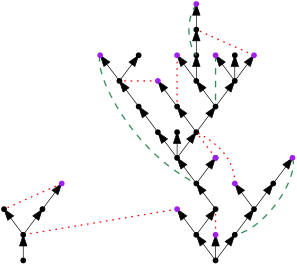
\includegraphics[width=0.7\linewidth]{Content/Pictures/Types of surplus edges.png}
    \caption{This figure illustrates an example of a depth-first exploration of two out-components with the different type of surplus edges highlighted. The ancestral surplus edges (green) point from a vertex $v$ to one of its ancentors. They are always part of a strongly connected component. The descendental surplus edges (blue) point from a vertex $v$ to one of its descendants.  Any other surplus edge (red) is called an additional surplus edge. Descendental and additional surplus edges are sometimes part of a strongly connected component.}
    \label{subfigure.typesofsurplusedges} 
\end{subfigure}\\
\begin{subfigure}{0.7\textwidth}
  \centering
  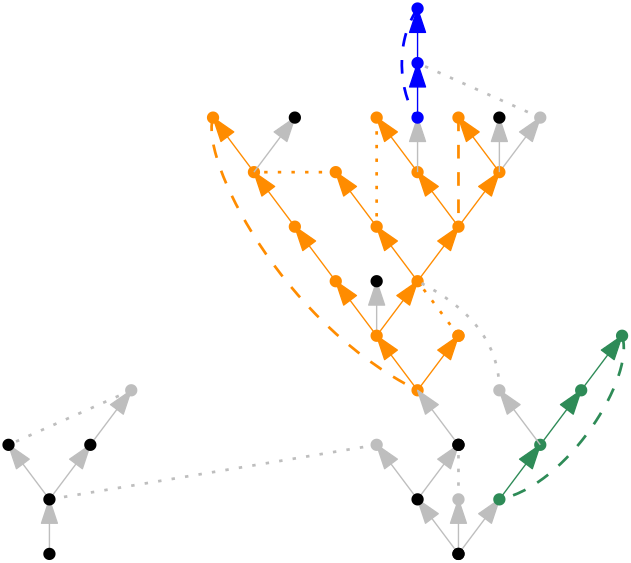
\includegraphics[width=0.7\linewidth]{Content/Pictures/SCC in example.png}
  \caption{The non-trivial strongly connected components embedded in the components of the out-forest are depicted in blue, green and orange. The trivial strongly connected components are black. The grey edges are not part of a strongly connected component, and the grey vertices correspond to purple leaves that are not part of a strongly connected component.}
    \label{subfigure.sccinexample}
\end{subfigure}
\caption{We illustrate the different types of surplus edges and how they affect the structure of the strongly connected components.}
\end{figure}

\subsection{Convergence of the positions of the ancestral surplus edges}\label{subsec.ancestral}
In this subsection, we will prove that the law of the position of the ancestral surplus edges converges under scaling. We will visit the purple vertices in depth-first order, and for every purple vertex we will sample whether its corresponding surplus edge is ancestral. The probability that a purple vertex corresponds to an ancestral surplus edge is given by the number of unpaired in-edges on its path to the root divided by the number of unpaired, seen in-edges. Therefore, to understand the distribution of the position of ancestral surplus edges, we need to understand where the unpaired in-edges are. We will study this by modifying the edge lengths in the tree: for a vertex with in-degree $m$, the edges connecting it to its children will have length $m-1$. The height of vertex $w$ in this forest with edge lengths approximately corresponds to the number of unpaired in-edges on the path from $w$ to the root. We add lengths to all edges in $(\hat{\cF}_n(k),k\geq 1)$ and call the resulting forest with edge lengths $(\hat{\cF}^\ell_n(k),k\geq 1)$. Denote the height process of $(\hat{\cF}^\ell_n(k),k\geq 1)$ by $\hat{H}_n^\ell(k)$. Then, we get the following extension of Theorem \ref{thm.convoutforest}.
\begin{lemma}\label{lemma.heightprocesswithlengths}
Let $(B_t)_{t\geq 0}$ be a Brownian motion, and define
$$(\hat{B}_t,t\geq 0):=\left( B_t-\frac{\sigma_{-+}+\nu_-}{2\sigma_+ \mu}t^2, t\geq 0\right).$$ Then,

\begin{align*}&\left(n^{-1/3}\hat{S}^{p,+}_n\left(\lfloor n^{2/3}t\rfloor \right),n^{-1/3}\hat{H}_{n}\left(\lfloor n^{2/3}t\rfloor \right),n^{-1/3}\hat{H}^\ell_{n}\left(\lfloor n^{2/3}t\rfloor \right),  t\geq 0\right)\\
&\overset{d}{\to}\left(\sigma_+ \hat{B}_t, \frac{2}{\sigma_+} \hat{R}_t,\frac{2(\sigma_{-+}+\nu_-)}{\sigma_+\mu} \hat{R}_t, t\geq 0\right)\end{align*}
in $\D(\R_+,\R)^3$, for 
$$(\hat{R}_t,t\geq 0)=\left(\hat{B}_t-\inf\left\{\hat{B}_s: s\leq t\right\},t\geq 0\right),$$
jointly with 
$$\left(n^{-2/3}\hat{S}_n^-\left(\lfloor n^{2/3}t\rfloor \right), n^{-1/3}\hat{P}_n\left(\lfloor n^{2/3}t\rfloor \right),t\geq 0\right)\overset{d}{\to}\left(\nu_-t,  \frac{\nu_-}{2\mu} t^2, t\geq 0\right)$$
in $\D(\R_+,\R)^2$ as $n\to \infty$.
\end{lemma}
\begin{proof}
We use Theorem 1 in \cite{deraphelisScalingLimitMultitype2017} by de Raphélis, that shows convergence of the height process of a Galton-Watson forest with edge-lengths under a few conditions on the degree and edge length distribution. We equip $(\cF^{pr}(k),k\geq 1)$, as defined in Subsubsection \ref{subsubsec.convheightprocess} with edge lengths, and apply the result. For a vertex in $(\cF^{pr}(k),k\geq 1)$ with degree $(d^+,d^-)$, let the edges connecting it to its children have length $d^--1$. Call the resulting forest with edge lengths $(\cF^{pr,\ell}(k),k\geq 1)$, and let $(H^{pr,\ell}(k),k\geq 1)$ be the corresponding height process. \myworries{Horrible notation. We don't use it elsewhere, so maybe it's okay to leave it like this} \myworries{Be more clear about what the 'in-degree' of a vertex in this forest is. The 'in-degree' of black and blue vertice is encoded by $S^-(k)$, and I need to define it for red vertices.} We will translate the conditions of Theorem 1 in \cite{deraphelisScalingLimitMultitype2017} to our setting and check them. The conditions are as follows.
\begin{enumerate}
    \item $\E[D^+(Z^-)]=1$
    \item $1<\E[(D^+(Z^-))^2]<\infty$
    \item $\E\left[D^+(Z^-)\one_{(Z^--1-1)>x}\right]=o(x^{-2})$ as $x\to \infty$
\end{enumerate}
Under these conditions, using the notation from Subsubsection \ref{subsubsec.convheightprocess},
\begin{align}\begin{split}\label{eq.convmodifiedheightprocess}
&\left(n^{-1/3}S^{pr,+}\left(\lfloor t n^{2/3}\rfloor \right),n^{-1/3}H^{pr}\left(\lfloor t n^{2/3}\rfloor \right), n^{-1/3}H^{pr,\ell}\left(\lfloor t n^{2/3}\rfloor \right),t\geq 0\right)\\
&\overset{d}{\to}\left(\sigma_+ B_s, \frac{2}{\sigma_+}\left(B_s-\inf\left\{B_u:u\leq s\right\}\right), \frac{2(\sigma_{+-}+\nu_-)}{\mu\sigma_+}\left(B_s-\inf\left\{B_u:u\leq s\right\}\right),t\geq 0\right)
\end{split}\end{align}
in $D(\R_+,\R)^3$ as $n\to \infty$. 
Then, we observe that the rest of the argument in Subsubsection \ref{subsubsec.convheightprocess} and Subsection \ref{subsubsec.convaftermeasurechange} can be extended to include the height process with edge lengths. This yields the result.\\
Therefore, to finish the proof, we need the conditions of Theorem 1 in \cite{deraphelisScalingLimitMultitype2017} to hold. The conditions are equivalent to 
\begin{enumerate}
    \item $\E[D^+D^-]=\E[D^-]$
    \item $1<\frac{\E[(D^+)^2D^-]}{\E[D^-]}<\infty$
    \item $\E\left[D^+D^-\one_{D^->x}\right]=o(x^{-2})$ as $x\to \infty$. 
\end{enumerate}
Note that the first and second condition follow directly from the assumptions, and the third condition is implied by $\E[D^+(D^-)^3]<\infty$.
\end{proof}\\

This lemma allows us to study the convergence of the position of the ancestral surplus edges. We use the following definitions. Let $N_n(k)$ denote the number of ancestral surplus edges found up to time $k$. Note that $N_n(k)-N_n(k-1)=1$ can only hold if $\hat{P}_n(k)-\hat{P}_n(k-1)=1$, i.e. if at time $k$, we visit a purple vertex. If $N_n(k)-N_n(k-1)=1$, i.e. if the purple vertex visited at time $k$ corresponds to an ancestral surplus edge, sample  the height of the vertex to which the surplus edge connects and denote it by $U^n(k)$. If $N_n(k)-N_n(k-1)=0$, declare $U^n(k)=\omega$. Note that by definition, an ancestral surplus edge formed at time $k$ always connects to a vertex on the path to the root from the vertex visited at time $k$, so its position is uniquely determined by the height on this path. We will show that the law of $(N^(k),U^n(k))$ converges under scaling, which is the content of the following theorem. 

\begin{theorem}\label{thm.convergenceancestraledges}
We have that, jointly with the convergence in Lemma \ref{lemma.heightprocesswithlengths},
\begin{align*}&\left(N_n\left(\lfloor tn^{2/3}\rfloor\right), n^{-1/3}U^n\left(\lfloor tn^{2/3}\rfloor\right),t\geq 0\right)\\
&\overset{d}{\to}\left(N_t,U_t,t\geq 0\right),\end{align*}
as $n\to \infty$, where $(N_t,U_t,t\geq 0)$ is a marked Cox process of intensity $$\frac{2(\sigma_{-+}+\nu_-)}{\sigma_+\mu^2} \hat{R}_t$$ at time $t$, and, in case of a jump at time $t$, the mark is uniform on $$[0,\frac{2}{\sigma_+} \hat{R}_t].$$ 
Here, the convergence is in $D(\R_+,\R)$ for the first coordinate, and in the topology of vague convergence for counting measures on $\R_+\cup \{\omega\}$ for the second. 
\end{theorem}
In the proof of Theorem \ref{thm.convergenceancestraledges} we use the following, straightforward, technical result.
\begin{lemma}\label{lemma.technicalcomposedfunctions}
If $h_n\to h$ and $f_n\to f$ in $\D(\R_+,\R)$ as $n\to\infty$, and $h_n$ and $h$ are monotone non-decreasing and $h$ is continuous, then 
$$h_n\circ f_n \to h\circ f$$
in $\D(\R_+,\R)$ as $n\to\infty$.
\end{lemma}
\begin{proof}
Using the characterization of convergence in the Skorokhod topology given in Proposition 3.6.5 in \cite{ethierMarkovProcessesCharacterization1986} by Ethier and Kurtz, the result follows immediately.
\end{proof}
We also make use of the following lemma, that we will prove after the proof of Theorem \ref{thm.convergenceancestraledges}. 
\begin{lemma}\label{lemma.usedancestralonpathtoroot}
For $k\leq \lfloor tn^{2/3}\rfloor$, let $E^t_n(k)$ denote the number of in-edges on the path to the root from the vertex visited at time $k$ that are part of a surplus edge at time $\lfloor tn^{2/3}\rfloor$. Then, for all $t>0$,
$$n^{-1/3}\max\left\{E^t_n(k):k\leq n^{2/3}t\right\}\overset{p}{\to}0$$
as $n\to \infty$.
\end{lemma}

\begin{proofof}{ Theorem \ref{thm.convergenceancestraledges}}
We note that $(N_n(k),k\geq 1)$ is a counting process with compensator 
\begin{align*}
    N_n^{comp}(k)&=\sum_{i=1}^k \one_{\{\hat{P}_n(i)-\hat{P}_n(i-1)=1\}}\frac{\hat{H}^\ell_n(i)+1-E_n(i)}{\hat{S}^-_n(i)}\\
    &=\sum_{j=1}^{\hat{P}_n(k)}\frac{\hat{H}^\ell_n(\min\{l:\hat{P}_n(l)\geq k\})-E(\min\{l:\hat{P}_n(l)\geq k\})}{\hat{S}^-_n(\min\{l:\hat{P}_n(l)\geq k\})},
\end{align*}
where $(E_n(k),k\geq 1)$ denotes the number of in-edges on the path to the root from the vertex visited at time $k$ that are part of a surplus edge at time $k$. Indeed, if vertex $i$ is purple, it will be paired with a uniform in-edge that is already seen, but unpaired, of which we have $\hat{S}^-_n(i)$ in total, and $\hat{H}^\ell_n(i)+1-E_n(i)$ of those form an ancestral surplus edge. By Theorem 14.2.VIII of Daley and Vere-Jones \cite{daleyIntroductionTheoryPoint2008}, the claimed convergence under rescaling of $(N_n(k),k\geq 1)$ follows if we show that 
\begin{equation}\label{eq.convergencecompensator}
    \left(N_n^{comp}\left(\lfloor tn^{2/3}\rfloor \right), t\geq 0\right)\overset{d}{\to}\left(\frac{2(\sigma_{-+}+\nu_-)}{\sigma_+\mu^2} \int_0^t\hat{R}_v dv, t \geq 0\right)
\end{equation}
in $\D(\R_+,\R)$ as $n\to \infty$ jointly with the convergence in Lemma \ref{lemma.heightprocesswithlengths}. Therefore, we will now prove that \eqref{eq.convergencecompensator} holds. 
Firstly, note that $E_n(k)\leq E_n^t(k)$, so we can use Lemma \ref{lemma.usedancestralonpathtoroot} to control this error term. Moreover, by
$$\left(n^{-1/3}\hat{P}_n\left(\lfloor n^{2/3}t\rfloor \right),t\geq 0\right)\overset{p}{\to}\left(\frac{\nu_-}{2\mu}t^2,t\geq 0\right)$$
in $\D(\R_+,\R)$ as $n\to \infty$,
we also get that
\begin{align*}\left(n^{-2/3}\min\{l\geq 1:n^{-1/3}\hat{P}_n(l)\geq t\},t\geq 0\right)&\overset{p}{\to}\left(\min\left\{s>0: \frac{\nu_-}{2\mu}s^2\geq t\right \}, t\geq 0\right)\\
&=:\left(p^{-1}(t),t\geq 0\right) \end{align*}
in $\D(\R_+,\R)$ as $n\to \infty$, because $\left(\frac{\nu_-}{2\mu}t^2,t\geq 0\right)$ is strictly increasing. Then, Lemma \ref{lemma.heightprocesswithlengths}, Lemma \ref{lemma.technicalcomposedfunctions}, Lemma \ref{lemma.usedancestralonpathtoroot}, Slutsky's lemma and the continuous mapping theorem imply that 
\begin{align*}&\left(\sum_{j=1}^{\lfloor n^{1/3}t\rfloor}\frac{\hat{H}^\ell_n(\min\{l:\hat{P}_n(l)\geq k\})-E(\min\{l:\hat{P}_n(l)\geq k\})}{\hat{S}^-_n(\min\{l:\hat{P}_n(l)\geq k\})},t\geq 0\right)\\
&\overset{d}{\to} \left( \frac{2(\sigma_{-+}+\nu_-)}{\sigma_+\mu} \int_0^t \frac{\hat{R}_{p^{-1}(s)}}{\nu_- p^{-1}(s)}ds,t\geq 0 \right).
\end{align*}
If we combine this with the convergence under rescaling of $(P_n(k),k\geq 1)$ and apply Lemma \ref{lemma.technicalcomposedfunctions}, some simple analysis then yields \eqref{eq.convergencecompensator}. \\
Finally, the position of the marks is uniform on the available in-edges on the path to the root. Therefore, since, asymptotically, on the scale that we are interested in, $(\hat{H}_n(k),k\leq \lfloor n^{2/3}t\rfloor)$ and $(\hat{H}_n(k),k\leq \lfloor n^{2/3}t\rfloor)$ only differ by a constant factor, the position of the marks in the limit is in fact uniform on the path to the root. 
\end{proofof}

\begin{proofof}{ Lemma \ref{lemma.usedancestralonpathtoroot}}
We need to show that for all $t>0$, $$n^{-1/3}\max \left\{E^t_n(k):k\leq n^{2/3} t \right\}\overset{p}{\to}0$$ as $n\to \infty$. Fix $\epsilon>0$. Note that the probability that a given in-edge of a vertex discovered before time $\lfloor t n^{2/3}\rfloor$ is part of a surplus edge before time $\lfloor t n^{2/3}\rfloor$ is bounded above by $$\frac{\sum_{i=1}^{\lfloor t n^{2/3}\rfloor} \hat{D}_i^+}{\sum_{i=1}^n D_i}.$$ Note that $$\left(n^{-1/3}\frac{\sum_{i=1}^{\lfloor t n^{2/3}\rfloor} \hat{D}_i^+}{\sum_{i=1}^n D_i}\right)_{n\geq 0}$$ is tight, so there exists a $c$ such that, with probability at least $1-\epsilon$, for every in-edge that is seen before time $\lfloor t n^{2/3}\rfloor$, the probability that it is part of a surplus edge before time $\lfloor t n^{2/3}\rfloor$ is bounded above $cn^{-1/3}$ for all $n$. Let $\mathcal{E}$ be the event that all these probabilities are bounded by $cn^{-1/3}$ for all $n$. Let $n$ be large enough such that $n^{-1/3}c\leq 1$. This means that on $\mathcal{E}$, there exists a coupling such that we can mark each in-edge with probability $n^{-1/3}c$ independently, such that the in-edges that are part of a surplus edge at time $\lfloor tn^{2/3}\rfloor$ are a subset of the marked in-edges. We claim that the maximum number of marked in-edges on a path to the root up to time $\lfloor n^{2/3}t\rfloor$ is $o(n^{1/3})$ in probability. Note that the number of marked vertices on the path to the root from the vertex visited at time $k$ is the sum of $\hat{H}^\ell_n(k)+1$ independent $\operatorname{Bernoulli}(cn^{-1/3})$ random variables. The sets of Bernoulli random variables that are counted at different times $k$ have a possibly non-empty intersection. To deal with this, we use the following fact. For $A_1,\dots, A_k$ i.i.d random variables and $B_1,\dots,B_k$ i.i.d. random variables, $\max_{i\leq k} (A_i+B_1)$ is stochastically dominated by $\max_{i\leq k}(A_i+B_i)$. Hence, the maximum number of marked in-edges on a path to the root up to time $\lfloor n^{2/3}t\rfloor$ is  stochastically dominated by $\max_{k\leq \lfloor n^{2/3} t \rfloor} B_k$, with the $B_k$ independent and $B_k\sim \operatorname{Binom}(H^\ell_{eff}(k)+1,n^{-1/3}c)$. However, we know that $\left(n^{-1/3}\max_{k\leq \lfloor tn^{2/3}\rfloor}H^\ell_{eff}(k)\right)_{n\geq 1}$ is tight, and for $A^n_1,A^n_2,\dots$ i.i.d. with $A^n_1\sim  \operatorname{Binom}(n^{1/3}K',n^{-1/3}c)$,
 $\max_{k\leq \lfloor n^{2/3} K \rfloor}A^n_k$ is of order $\log(n)/\log(\log(n))$, which proves the statement.
\end{proofof}
\subsection{Extracting the important components of the out-forest}
In this subsection, we will show that, conditional on the convergence under rescaling that is shown in Theorem \ref{thm.convergenceancestraledges}, the sequence of components in $(\hat{\cF}_n(k),k\leq \lfloor n^{2/3}t)$ that contain ancestral surplus edges converges as well under rescaling. Lemma \ref{lemma.extractexcursions} is a statement about extracting excursions from deterministic functions with marks, which we will apply to the sample paths of $(\hat{S}_n^{p,+}(k),k\geq 1)$ decorated with the marks given by $(N_n(k),U_n(k))$. The lemma tells us that if the sample paths and marks converge, the beginnings and endpoints of the excursions above the running infimum that contain the marks converge as well. \myworries{Revise this text at a later time} 
\begin{lemma}\label{lemma.extractexcursions}
Let $(f_n(t), t\geq 0)$ for $n\geq 1$, and $(f(t),t\geq 0)$ be functions in $\D(\R_+,\R)$, such that 
$$(f_n(t), t\geq 0)\to (f(t),t\geq 0)$$ in $\D(\R_+,\R)$ as $n\to \infty$. Assume that $(f(t),t\geq 0)$ is continuous, that $f(t)\to -\infty$ as $t\to \infty$, and that the local minima of $(f(t),t\geq 0)$ are unique. Moreover, let $(x_i^n,y_i^n)_{1\leq i\leq m}$, for $n\geq 1$, and $(x_i,y_i)_{1\leq i\leq m}$ be elements of $\R^{2m}$ such that for all $i\in [m]$, $(x_i^n,y_i^n)\to (x_i,y_i)$ in $\R^2$ as $n\to \infty$, and such that $f(x_i)-\inf\{f(s):s\leq x_i\}>0$ for all $i\in [m]$. Define
\begin{align*}g_i^n&=\inf\left\{t\geq 0:f_n(t)=\inf\{f_n(s):s\leq x_i^n\}\right\}\text{ for }i\in [m]\text{, }n\geq 1\\
d_i^n&=\inf\left\{ t\geq 0: \inf\{f_n(s):s\leq t\} < \inf\{f_n(s):s\leq x_i^n\}\right\}\text{ for }i\in [m]\text{, }n\geq 1\\
g_i&=\inf\left\{t\geq 0:f(t)=\inf\{f(s):s\leq x_i\}\right\},\text{ and}\\
d_i&=\inf\left\{ t\geq 0: \inf\{f(s):s\leq t\} < \inf\{f(s):s\leq x_i\}\right\}.
\end{align*}
Define $\sigma^i_n=d_i^n-g_i^n$, for $i\in [m]$, $n\geq 1$ and $\sigma^i=d_i-g_i$. Assume $g_i\neq g_j\implies \sigma_i\neq \sigma_j$. For $S=\{(a_i,b_i,c_i), i\in [m]\}$, let $\operatorname{ord}(S)$ be a sequence consisting of the elements of $S$ put in decreasing order of $a_i$, with ties broken arbitrarily, and concatenated with $(0,0,0)_{i\geq 1}$ such that $\operatorname{ord}(S)\in (\R^3)^\infty$. Then, 
$$\operatorname{ord}\left(\left\{(\sigma_i^n,g_i^n,d_i^n):1\leq i \leq m\right\}\right)\to \operatorname{ord}\left(\left\{(\sigma_i,g_i,d_i):1\leq i \leq m\right\}\right)$$
in $(\R^{3})^\infty$ in the $\ell_1$-topology as $n\to \infty$. 
\end{lemma}
\begin{proof}
First, note that $g_i^n$, $d_i^n$, $g_i$, and $d_i$ are well-defined for all $i\in [m]$, $n\geq 1$ by $f(t)\to -\infty$ as $t\to \infty$ and convergence of $f_n$ to $f$. \\
Fix $i$. We will first show that $g^n_i\to g_i$ and $d_i^n\to d_i$ as $n\to \infty$. Firstly, note that by the assumption that $f(x_i)-\inf\{f(s):s\leq x_i\}>0$ and the continuity of $f$, $g_i<x_i<d_i$. Fix $0<\epsilon<\min\{x_i-g_i,d_i-x_i\}/2$. We claim that the following conditions are sufficient for $g^n_i\to g_i$ and $d_i^n\to d_i$ as $n\to \infty$
\begin{enumerate}
    \item \label{cond.excursions1} $g_i+\epsilon<x^n_i<d_i-\epsilon$
    \item \label{cond.excursions2}$\inf\left\{f_n(s):s\in (g_i-\epsilon, g_i+\epsilon)\right\}<\inf\left\{f_n(s):s\in [g_i+\epsilon,d_i-\epsilon] \right\}$, 
    \item \label{cond.excursions3}$\inf\left\{f_n(s):s\in (g_i-\epsilon, g_i+\epsilon)\right\}<\inf\left\{f_n(s):s\in [0,g_i-\epsilon]\right\}$,
    \item \label{cond.excursions4} $\inf\left\{ f_n(s):s\in (d_i-\epsilon,d_i+\epsilon)\right\}<\inf\left\{f_n(s):s\in [0,d_i-\epsilon]\right\}$
\end{enumerate}
for all $n$ large enough. Indeed, condition \ref{cond.excursions1}, \ref{cond.excursions2} and \ref{cond.excursions3} imply $|g^n_i-g_i|<\epsilon$, while condition \ref{cond.excursions1}, \ref{cond.excursions2} and \ref{cond.excursions4} imply $|d^n_i-d_i|<\epsilon$. Note that condition \ref{cond.excursions1} holds for $n$ large enough by definition of $\epsilon$ and convergence of $x_i^n$ to $x_i$. To show the other conditions, define
\begin{align*}\delta_1&=\inf\left\{f(s):s\in [g_i+\epsilon,d_i-\epsilon]\right\}-\inf\left\{f(s):s\in (g_i-\epsilon,g_i+\epsilon)\right\}\\
\delta_2&=\inf\left\{f(s):s\in [0,g_i-\epsilon]\right\}-\inf\left\{f(s):s\in (g_i-\epsilon,g_i+\epsilon)\right\}\\
\delta_3&=\inf\left\{f(s):s\in [0,d_i-\epsilon]\right\}-\inf\left\{f(s):s\in (d_i-\epsilon,d_i+\epsilon)\right\}
\end{align*}
By uniqueness of local minima and the definition of $g_i$ and $d_i$,  $\delta:=\min\{\delta_1,\delta_2,\delta_3\}/3>0$. Then, note that for $n$ large enough, $\sup\{|f_n(s)-f(s)|:s\leq g_i+\epsilon\}<\delta$, which implies conditions \ref{cond.excursions2}, \ref{cond.excursions3}, and \ref{cond.excursions4} for such $n$. \\
Since $i$ was arbitrary, and $m$ is finite, we find that 
$$(x_i^n,y_i^n)_{1\leq i\leq m}\to (x_i,y_i)_{1\leq i\leq m}$$
in $\R^{2m}$ as $n\to \infty$. \\
We now claim that $g_i^n\to g_i$ and $g_j^n\to g_i$ implies that $g_i^n=g_j^n$ for $n$ large enough. Indeed, by definition of $g_i^n$, $g_j^n$ and $\sigma_i^n$, we see that $g_i^n<g_j^n$ implies that $g_j^n-g_i^n\geq \sigma_i^n$, and by the argument above, $\sigma_i^n\to \sigma_i>0$, so $g_i^n-g^n_j\to 0$ can only hold if $g_i^n=g_j^n$ for $n$ large enough. The equivalent statement can be proved for $d_i^n$, which implies that 
$$\#\left\{(\sigma_i^n,g_i^n,d_i^n):1\leq i \leq m\right\}\to \#\left\{(\sigma_i,g_i,d_i):1\leq i \leq m\right\}.$$
We note that $\sigma^n_i\to \sigma_i$ for all $i$, so  $\sigma_i<\sigma_j$ implies that $\sigma^n_i<\sigma^n_j$ for all $n$ large enough. Then, using that, by assumption, $g_i\neq g_j$  implies that $\sigma_i\neq \sigma_j$, we get that
$$\operatorname{ord}\left(\left\{(\sigma_i^n,g_i^n,d_i^n):1\leq i \leq m\right\}\right)\to \operatorname{ord}\left(\left\{(\sigma_i,g_i,d_i):1\leq i \leq m\right\}\right)$$
in $(\R^{3})^\infty$ as $n\to \infty$.
\end{proof}

We now apply this result to our process to extract the excursion intervals that contain the marks representing ancestral backedges.
\begin{proposition}\label{prop.extractexcursions}
Fix $T>0$. Use notation as before. For $i\in \left[N_n\left(\lfloor T n^{2/3}\rfloor\right)\right]$, set $X_i^n=\min\{k:N_n(k)=i\}$, and $Y_i^n=U_n(X_i^n)$. Similarly, for $i$ in $\left[N(T)\right]$, set $X_i=\min\{t:N(t)=i\}$, and $Y_i=U(X_i)$. Define
\begin{align*}G_i^n&=\min\left\{k\geq 1:\hat{S}^{p,+}_n(k)=\min\{\hat{S}^{p,+}_n(l):l\leq X_i^n\}\right\}\text{ for }i\in \left[N_n\left(\lfloor T n^{2/3}\rfloor\right)\right]\text{, }n\geq 1\\
D_i^n&=\min\left\{k \geq 1: \min\left\{\hat{S}^{p,+}_n(l):l\leq k\right\} < \min\left\{\hat{S}^{p,+}_n(l):l\leq X_i^n\right\}\right\}\text{ for }i\in \left[N_n\left(\lfloor T n^{2/3}\rfloor\right)\right]\text{, }n\geq 1\\
G_i&=\inf\left\{t\geq 0:\sigma_+\hat{B}_t=\inf\{\sigma_+\hat{B}_s:s\leq X_i\}\right\},\text{ and}\\
D_i&=\inf\left\{ t\geq 0: \inf\{\sigma_+\hat{B}_s:s\leq t\} < \inf\{\sigma_+\hat{B}_s:s\leq X_i\}\right\}.
\end{align*}
Define $\Sigma_i^n=D_i^n-G_i^n$ and $\Sigma_i=D_i-G_i$. Then, for $\operatorname{ord}$ defined as in the statement of Lemma \ref{lemma.extractexcursions}, we get that
$$\operatorname{ord}\left(\left\{\left(n^{-2/3}\Sigma_i^n,n^{-2/3}G_i^n,n^{-2/3}D_i^n\right):1\leq i \leq N_n\left(\lfloor T n^{2/3}\rfloor\right)\right\}\right)\overset{d}{\to} \operatorname{ord}\left(\left\{(\Sigma_i,G_i,D_i):1\leq i \leq N(T)\right\}\right)$$
in the $\ell_1$-topology on $(\R^3)^\infty$ as $n\to \infty$, jointly with the convergence in Theorem \ref{thm.convergenceancestraledges}. 
\end{proposition}
\begin{proof}
We work on a probability space where the convergence in Theorem \ref{thm.convergenceancestraledges} holds almost surely, and claim that we can apply Lemma \ref{lemma.extractexcursions} to the sample paths of $\left(n^{-1/3}\hat{S}^{+,p}_n\left(\lfloor n^{2/3}t\rfloor\right),t \geq 0\right)$ with marks $$\left(n^{-2/3}X_n^i,n^{-1/3}Y_n^i\right)_{1\leq i\leq N_n\left(\lfloor T n^{2/3}\rfloor\right)}.$$ We check the conditions.
Firstly, note that by $N_n\left(\lfloor T n^{2/3}\rfloor\right)\to N\left(T\right)$ almost surely as $n\to \infty$, we can pick $n$ large enough such that $N_n\left(\lfloor T n^{2/3}\rfloor\right)=N\left(T\right)$, where we ignore events of $0$ probability. Furthermore, we observe that $(\hat{B}_t,t\geq 0)$ is a Brownian motion with negative parabolic drift, so the sample paths of $(\sigma_+\hat{B}_t,t\geq 0)$ are continuous and drift to $-\infty$ almost surely. By the local absolute continuity of $(\hat{B}_t,t\geq 0)$ to a Brownian motion, its local minima are almost surely unique, and the lengths of its excursions above the running infimum are all distinct. By 
$$\left(N_n\left(\lfloor t n^{2/3}\rfloor\right), n^{-1/3}U_n\left(\lfloor t n^{2/3}\rfloor\right), t\leq T\right) \overset{a.s.}{\to}\left(N\left(t\right), U\left(t\right),t\geq 0\right)$$
as $n\to \infty$, we observe that for all $i\in [N(T)]$, $(n^{-2/3}X_i^n,n^{-1/3}Y_i^n)\to (X_i,Y_i)$ almost surely in $\R^2$ as $n\to \infty$. The fact that $\hat{R}_{X_i}-\inf\{\hat{R}_s:s\leq X_i\}>0$ for all $i$ almost surely follows from the intensity of $(N_t,t\geq 0)$ at time $t$ being proportional to $\hat{R}_t$. This allows us to apply Lemma \ref{lemma.extractexcursions}, and the convergence follows.
\end{proof}

Given the convergence of the excursion intervals that contain the marks, it is straightforward to obtain convergence of the encoding processes of the components of $(\hat{\cF}_n(k), k\geq 1)$ that contain the marks. 
\begin{corollary}\label{cor.convergencesequenceofcomponents}
Recall notation in the statement of Proposition \ref{prop.extractexcursions}. For $i\in \left[N_n\left(\lfloor T n^{2/3}\rfloor\right)\right]$, set
\begin{align*}
    &\left(\mathsf{h}_i^n,\mathsf{h}_i^{\ell,n}, \mathsf{s}_i^{-,n}, \mathsf{p}^n_i, \mathsf{n}_i^n, \mathsf{u}_i^n\right)\\
    &=\left(n^{-1/3}\hat{H}_n\left(G_i^n+\lfloor n^{2/3} t \rfloor\right),n^{-1/3}\hat{H}^{\ell}_n\left(G_i^n+\lfloor n^{2/3} t \rfloor\right),  n^{-2/3}\hat{S}^{p,-}_n\left(G_i^n+\lfloor n^{2/3} t \rfloor\right),\right.\\
     &\qquad n^{-1/3}\left(\hat{P}_n\left(G_i^n+\lfloor n^{2/3} t \rfloor\right)-\hat{P}_n\left(G_i^n\right)\right), \hat{N}_n\left(G_i^n+\lfloor n^{2/3} t \rfloor\right)-\hat{N}_n\left(G_i^n\right), \\
     &\qquad \left.n^{-1/3}\hat{U}_n\left(G_i^n+\lfloor n^{2/3} t \rfloor\right), 0\leq t \leq n^{-2/3}\Sigma_i^n\right),
\end{align*}
such that $\left(\mathsf{h}_i^n,\mathsf{h}_i^{\ell,n}, \mathsf{s}_i^{-,n}, \mathsf{p}^n_i, \mathsf{n}_i^n, \mathsf{u}_i^n\right)$ encodes the marked component of $(\hat{\cF}_n(k), k\geq 1)$ that contains the $i^{th}$ ancestral surplus edge in depth-first order. 
Similarly, set
\begin{align*}
    &\left(\mathsf{h}_i,\mathsf{h}_i^{\ell}, \mathsf{s}_i^{-}, \mathsf{p}_i, \mathsf{n}_i, \mathsf{u}_i\right)\\
    &=\left(\frac{2}{\sigma_+}\hat{R}_{G_i+t},\frac{2(\sigma_{-+}+\nu_-)}{\sigma_+\mu}\hat{R}_{G_i+t},  \nu_-(G_i+t),\frac{\nu_-}{2\mu}\left((G_i+t)^2-G_i^2\right),\right.\\
    &\qquad\left.N(G_i+t)-N(G_i), U(G_i+t), 0\leq t \leq \Sigma_i\right).
\end{align*}
For $S=\{(a_i,\mathbf{b}_i), i\in [m]\}$, let $\operatorname{ord}(S)$ be a sequence consisting of the elements of $S$ put in decreasing order of $a_i$, with ties broken arbitrarily, and concatenated with $(0,\mathbf{0})_{i\geq 1}$.\\
Then, 
\begin{align*}&\operatorname{ord}\left(\left\{\Sigma_i^n, \left(\mathsf{h}_i^n,\mathsf{h}_i^{\ell,n}, \mathsf{s}_i^{-,n}, \mathsf{p}^n_i, \mathsf{n}_i^n, \mathsf{u}_i^n\right), i\in \left[N_n\left(\lfloor T n^{2/3}\rfloor\right)\right]\right\}\right)\\
&\overset{d}{\to}\operatorname{ord}\left(\left\{\Sigma_i, \left(\mathsf{h}_i,\mathsf{h}_i^{\ell}, \mathsf{s}_i^{-}, \mathsf{p}_i, \mathsf{n}_i, \mathsf{u}_i\right), i\in \left[N(T)\right]\right\}\right)\end{align*}
as $n\to \infty$. The topology on cadlag functions of the form $(f(t),t\leq a)$ is given by embedding the functions in $D(\R_+,\R)$ by considering $(\tilde{f}(t),t\geq 0)=(f(t)\one_{t<a}, t\geq 0)$. Then, we use the $\ell_1$-topology on the sequence space.
\end{corollary}
\begin{proof}
This is a consequence of Theorem \ref{thm.convergenceancestraledges} and Proposition \ref{prop.extractexcursions}. 
\end{proof}

\subsection{Convergence of the position of other important surplus edges}
As discussed in Subsection \ref{subsec.categoriessurplusedged}, ancestral surplus edges are important building blocks of non-trivial strongly connected components, but also descendental and additional surplus edges can be included in a strongly connected component. However, this can only occur if there is also an ancestral surplus edge present in the same strongly connected components. Corollary \ref{cor.convergencesequenceofcomponents} implies that the encoding processes of these components converge as a sequence ordered by component size (note that we include the purple vertices in the size). We will now define the process of finding the important additional and descendental surplus edges on such a component, given its encoding processes.\\
We will identify purple vertices that do not correspond to ancestral surplus edges, but are possibly part of a strongly connected component. We call these surplus edges \emph{candidates} and we define them in such a way that the important non-ancestral surplus edges are contained in the set of candidates. We will use Lemma \ref{lemma.whatispartofscc}.\ref{item.factsonsccs4} to define our candidates. The lemma states that non-ancestral surplus edges are only important if their endpoint is on the path from the root of the out-component to the starting point of an important surplus edge. This is not a sufficient condition, but by only declaring a surplus edge a candidate if it is on the path from the root of the out-component to the starting point of another candidate, we will with high probability have a finite number of candidates per component, after which we can easily distinguish between candidates and important surplus edges.\\
\subsubsection{Identifying the candidates}
The procedure for finding candidates is as follows. Suppose we are given a finite tree $\cT$ with root $\rho$ and with $|\cT|$ vertices in total, in which the vertices are assigned indices in depth-first order, and in which some of the leaves are coloured purple. Moreover, suppose we have a set of marks $A=\left\{(x_i,y_i):1\leq i \leq m\right\}\subset \left(\{1,\dots,\cT\}\times \N\right)^m$ such that for each $i$ vertex $x_i$ is purple. These marks correspond to the ancestral surplus edges in the tree. We also set $A_k=\left\{(x_i,y_i):x_i\leq k, 1\leq i \leq m\right\}$. Let be $C_k$ the candidates found before time $k$. Then, for $B=\{(a_1,b_1),\dots,(a_k,b_k)\}$ a subset of $[0,|\cT|]\times \N$, let $\cT(B)$ be the subtree of $\cT$ spanned by $\{\rho,a_1,\dots,a_k\}$. We define the active graph at time $k$ to be $\cG_k=\cT(A_k\cup C_k)\backslash \cT(\{k\})$. Note that by the argument above, a non-ancestral surplus edge visited at time $k$ should be declared a candidate if and only if its endpoint is in $\cG_k$. \\
We need extra information to determine the probability that the endpoint of a non-ancestral surplus edge visited at time $k$ has its endpoint in $\cG_k$. Like in Subsection \ref{subsec.ancestral}, we equip $\cT$ with edge lengths to encode the number of in-edges of vertices in $\cT$. Denote the resulting tree by $\cT^\ell$, and for a subgraph $\cG$ of $\cT$, let $\cG^\ell$ be equal to $\cG$ seen as a subtree of $\cT^\ell$ and let $\ell(\cG)$ the total length of $\cG^\ell$. In our model, $\cT$ will play the rôle of one tree in a forest, and we need information on trees explored before $\cT$, because surplus edges can also connect to those trees. We encode this with a process $(\mathsf{s}^-_{|\cT|}(k),1\leq k \leq |\cT|)$, that encodes the total number of seen available in-edges, such that $\mathsf{s}^-_{|\cT|}(0)$ represents the number of available in-edges in components explored before $\cT$ when we start the exploration of $\cT$. Then, the procedure is defined as follows. Perform the following iterative procedure for $k\in(1,\dots, |\cT|)$. Set $C_1=\emptyset$.
\begin{enumerate}
    \item If $k$ is not purple, or $(k,y)\in A_k$ for some $y$, set $C_k=C_{k+1}$.
    \item Otherwise, with probability 
    $$\frac{\ell(\cG_k)}{\mathsf{s}^-_{|\cT|}(k)}$$
    declare $k$ a candidate. Pick a uniform point in $\cG^\ell$ according to the length measure, and let $y$ be the first vertex on the path to $\rho$ from this point. Set $C_{k+1}=C_k\cup\{(k,y)\}$
\end{enumerate}
Set $C(\cT)=C_{|\cT|}$. 



\subsubsection{Convergence of the positions of the candidates}
\begin{proposition}

\end{proposition}





% For each $n\in \N$, fix $\sigma_n \in \R$, and let $\left(\mathsf{h}^n,\mathsf{h}^{\ell,n}, \mathsf{s}^{-,n}, \mathsf{p}^n, \mathsf{n}^n, \mathsf{u}^n\right)$ be a function from $[0,\sigma_n]$ to $\R_+^4\times \N \times (\R_+\cup \{\omega\})$. Similarly, let $\sigma \in \R$, and let $\left(\mathsf{h},\mathsf{h}^{\ell}, \mathsf{s}^{-}, \mathsf{p}, \mathsf{n}, \mathsf{u}\right)$ be a function from $[0,\sigma]$ to $\R_+^4\times \N \times (\R_+\cup \{\omega\})$. Assume that $\mathsf{n}^n$, $\mathsf{p}^n$, $\mathsf{n}$ and $\mathsf{p}$ are increasing functions that satisfy $\mathsf{n}^n(0)=\mathsf{p}^n(0)=\mathsf{n}(0)=\mathsf{p}(0)=0$. Also assume that $\mathsf{n}^n$ and $\mathsf{n}$ have increments of size $1$, and that $\mathsf{u}^n(t)\neq \omega$ if and only if $\mathsf{n}^n(t)-\mathsf{n}^n(t-)=1$, in which case $$\mathsf{u}^n(t)<\mathsf{h}^{n}(t)$, and similarly, that $\mathsf{u}(t)\neq \omega$ if and only if $\mathsf{n}(t)-\mathsf{n}(t-)=1$, in which case $$\mathsf{u}(t)<\mathsf{h}(t)$. Suppose that

\subsubsection{Important surplus edges on a single tree}



\subsection{For large $T$, we see all SCCs with large length before time $Tn^{2/3}$ with high probability}
We claim that exploring the out-components up to time $O(n^{2/3})$ is sufficient to see all large components. This is the content of the following theorem. The proof is in the same spirit as Lemma 9 in \cite{aldous_1991} by Aldous. 
\begin{lemma}
For $\delta>0$ and $I$ an interval, let $SCC(n,I,\delta)$ denote the number of SCCs whose vertices have at total of at least $\delta n^{1/3}$ in-edges and whose time of first discovery is in $n^{2/3}I$. Then,
$$\lim_{s\to \infty}\limsup_{n} \P\left(SCC(n,(s,\infty),\delta)\geq 1\right)=0\text{ for all }\delta>0.$$
\end{lemma}
\begin{proof}
Fix $\delta>0$. Suppose there is a strongly connected component $C$ with $vn^{1/3}$ total in-edges. Conditional on this fact, the in-edges that are paired up to the first in-edge of $C$ is paired, are uniform picks (without replacement) from the total set of in-edges. Denote the time of discovery of the first in-edge of $C$ times $n^{-2/3}$ by $\Xi_n$. Then, $\Xi_n\overset{d}{\to}\operatorname{Exp}(v)$. Fix $\epsilon>0$. We see that, by the memoryless property at time $s$,
$$\P\left(SCC\left(n,(s,2s),\delta\right)=0|SCC\left(n,(s,\infty),\delta\right)\geq 1\right)$$
is asymptotically bounded from above by 
$\exp(-s\delta)$, such that we can find an $s>0$ such that for all $n$ large enough,
$$\P\left(SCC\left(n,(s,\infty),\delta\right)\geq 1 \text{ and }SCC\left(n,(s,2s),\delta\right)=0\right)<\epsilon.$$
We claim that, by possibly increasing $s$ and $n$, we also get that 
$$\P\left(SCC\left(n,(s,2s),\delta\right)=0\right)>1-\epsilon,$$
which proves the statement.
Firstly, note that it is clear from the description of the limit process that, for $s$ large enough, with probability at most $\epsilon/2$, an SCC with total length at least \myworries{$\delta$ divided by ratio in-edges count vs length} is discovered after time $s$. By convergence of the exploration process on compact time intervals, by choosing $n$ large enough, we can then ensure that 
$$\P\left(SCC\left(n,(s,2s),\delta\right)=0\right)>1-\epsilon.$$
We conclude that 
$$\P(SCC\left(n,(s,\infty),\delta\right)\geq 1)\leq 2\epsilon.$$
\end{proof}
\subsection{Convergence of the cutting procedure}